\section{Database storage}
\label{sec:database}

The \textit{viaappiadb} database is running in the Via Appia Linux server.

The database logical scheme has conceptually two major parts: (a.) data management
information and (b.) the attribute data. The  data management part has 4 categories:
{\em ITEM}, {\em RAW}, {\em POTREE} and {\em OSG} and the attribute data is represented in the category {\em ATTRIBUTE}.
 
Figure \ref{fig:db_erdb} contains the Entity-Relationship diagram (ERD) of the
\textit{viaappiadb}. In the coming sections each category is described briefly and
illustrated. The direct connections between each category are also illustrated.

Note that some of the nodes of the relationships are \textit{0:n} or
\textit{0:1} (with black points) instead of the usual \textit{1:n} or
\textit{1:1}. This is to illustrate that some sites and objects may have
entries in some tables but not in others. For example it is possible to have a
site in the item table which has no entry in the attributes table (tbl1\_site) because attribute information of that site has not been collected yet.

\begin{figure}[H]
\centering
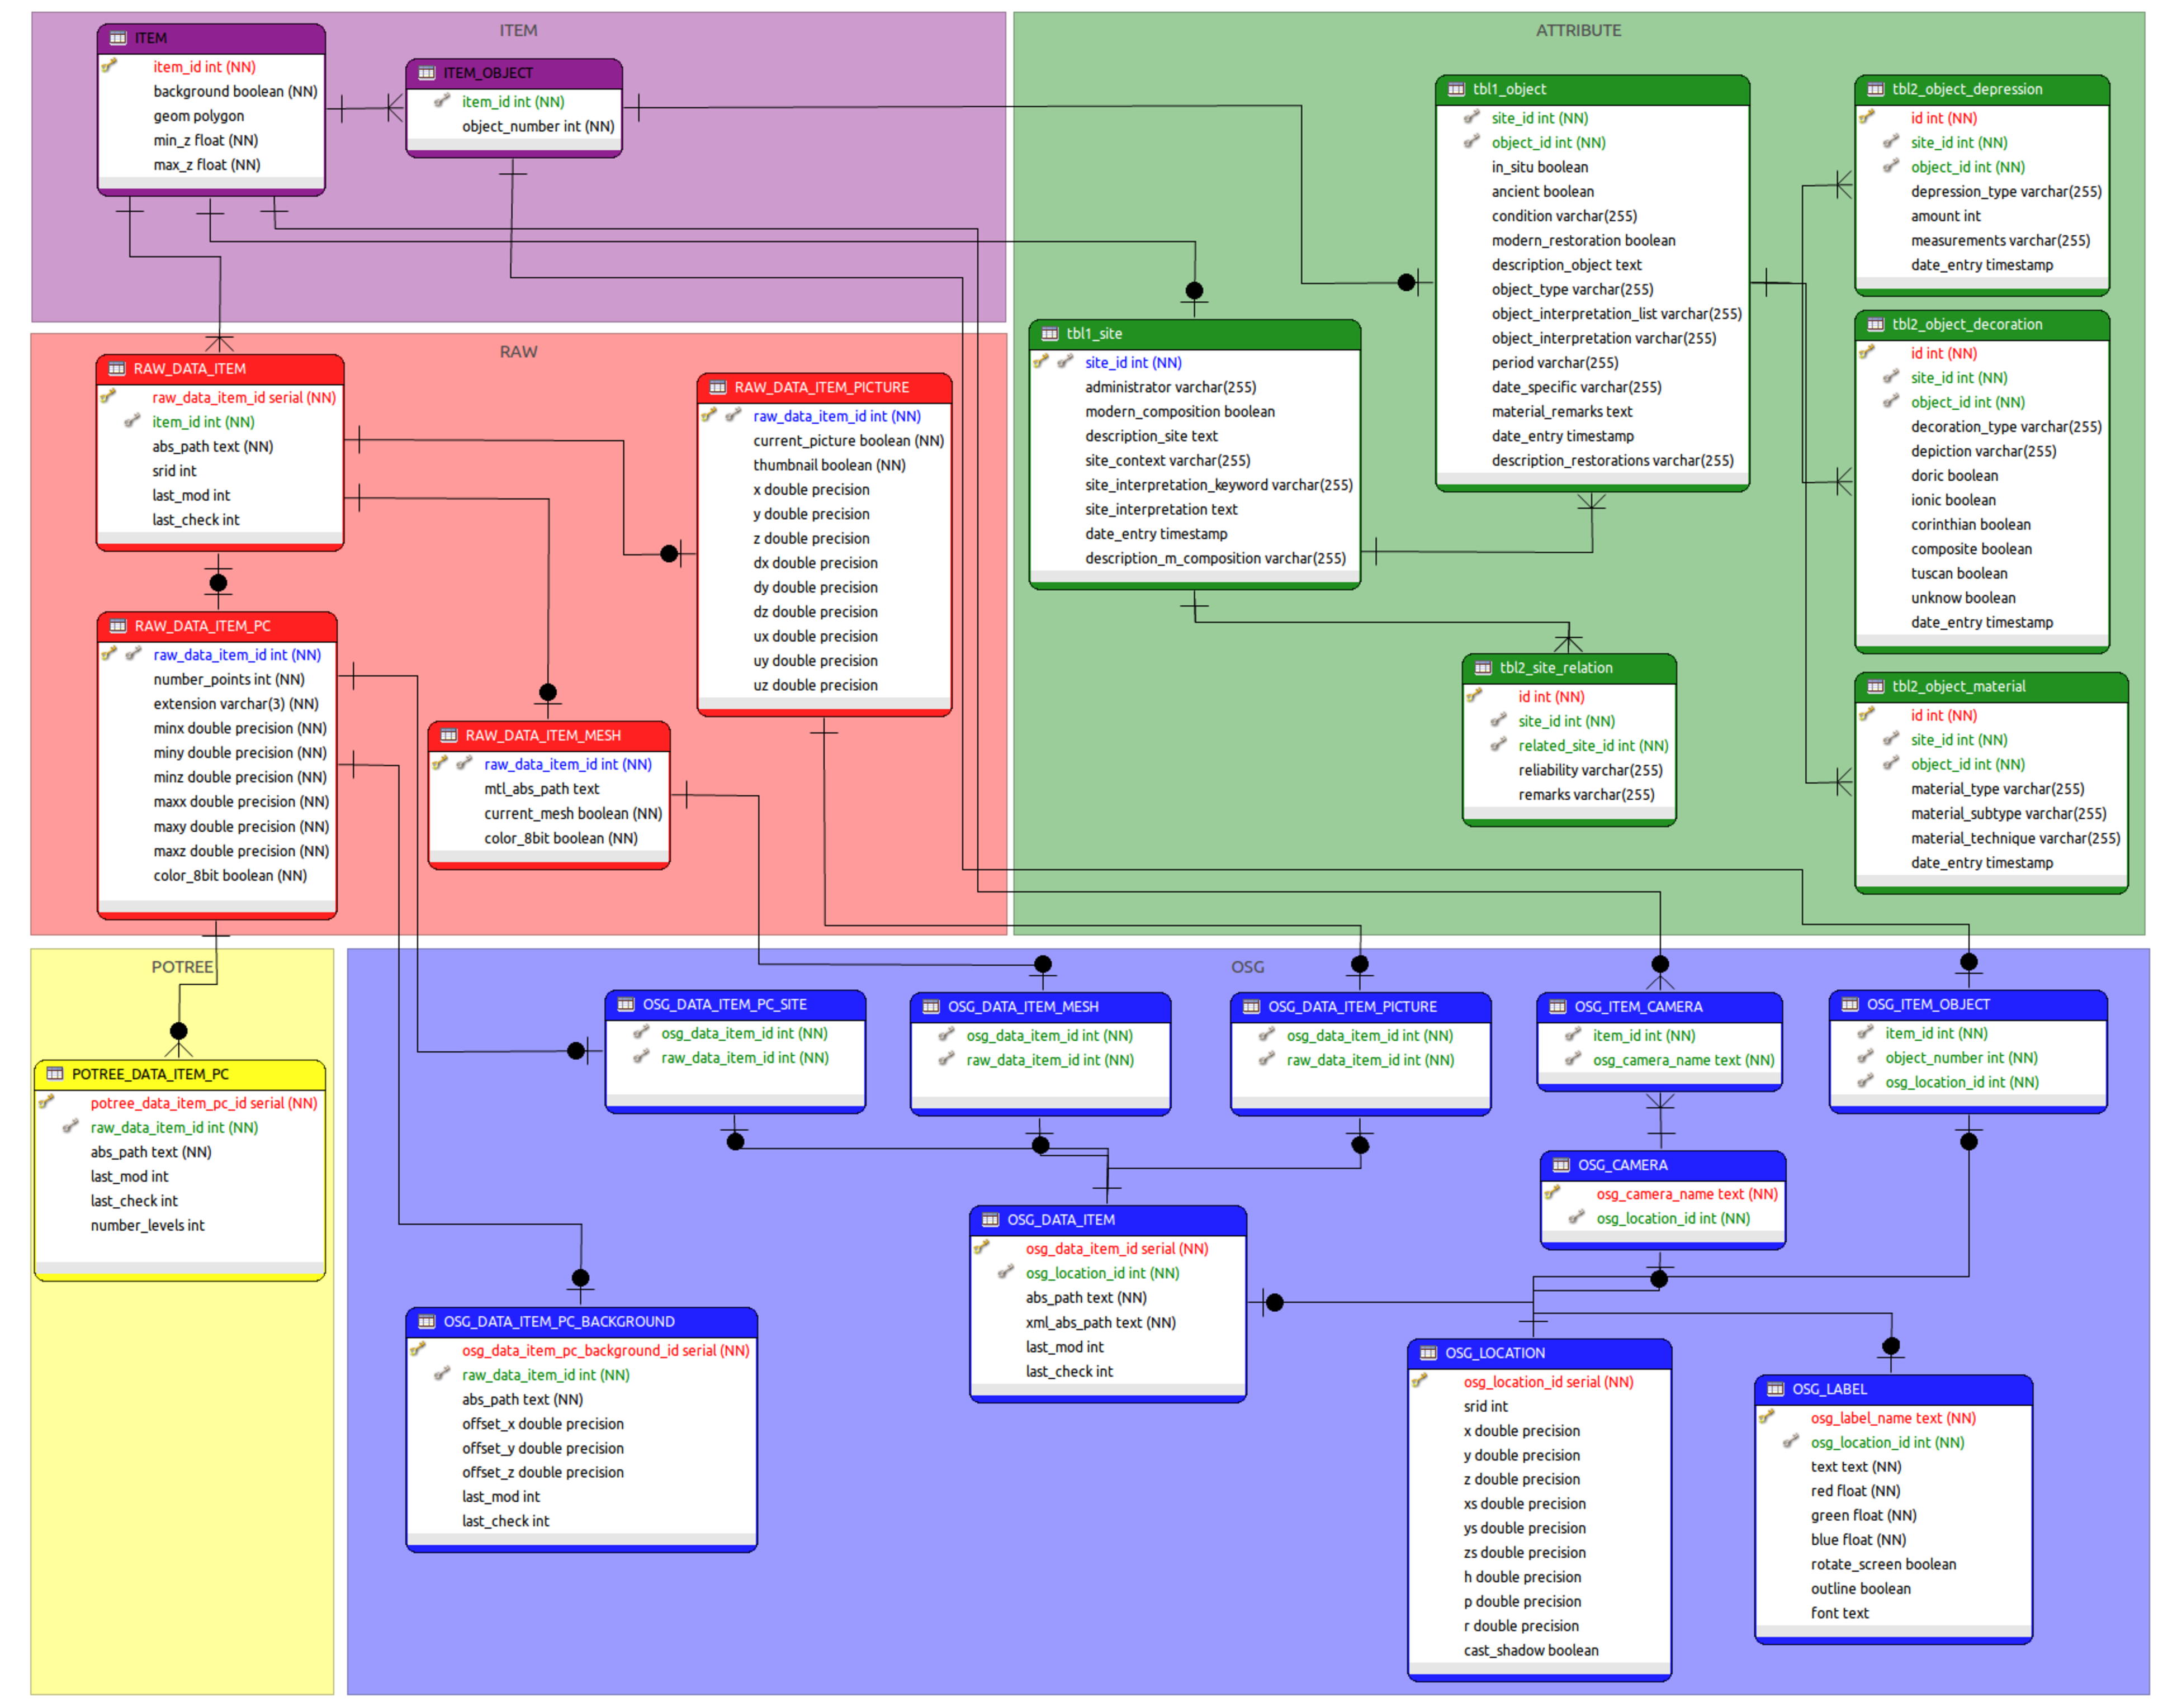
\includegraphics[scale=0.25]{fig/database/ERDB.pdf}
\caption{Entity-Relationship diagram of the \textit{viaappiadb} database with
its five categories.}
\label{fig:db_erdb}
\end{figure}

\subsection{Data management information}
This section describes the data management information related categories and for each category we detail its tables.

\subsubsection{ITEM}
{\em ITEM} is a category containing information about the {\em items} in the studied area.
As previously described, an {\em item} is any entity of interest and it can be either an archaeological site/monument or a background. We use the term background to identify the whole area where the archaeological sites are located. If the item of interest is an archaeological site, in which case the value of the logical field {\em background} is set to false, the different parts of the item are described as {\em item\_objects} and they are identified by the field {\em object\_number}. 

Figure \ref{fig:db_erdb_item} shows the relationship of the {\em ITEM} category with
the other categories. The {\em ITEM} category is on the top of the categories hierarchy.

\begin{figure}[H]
\centering
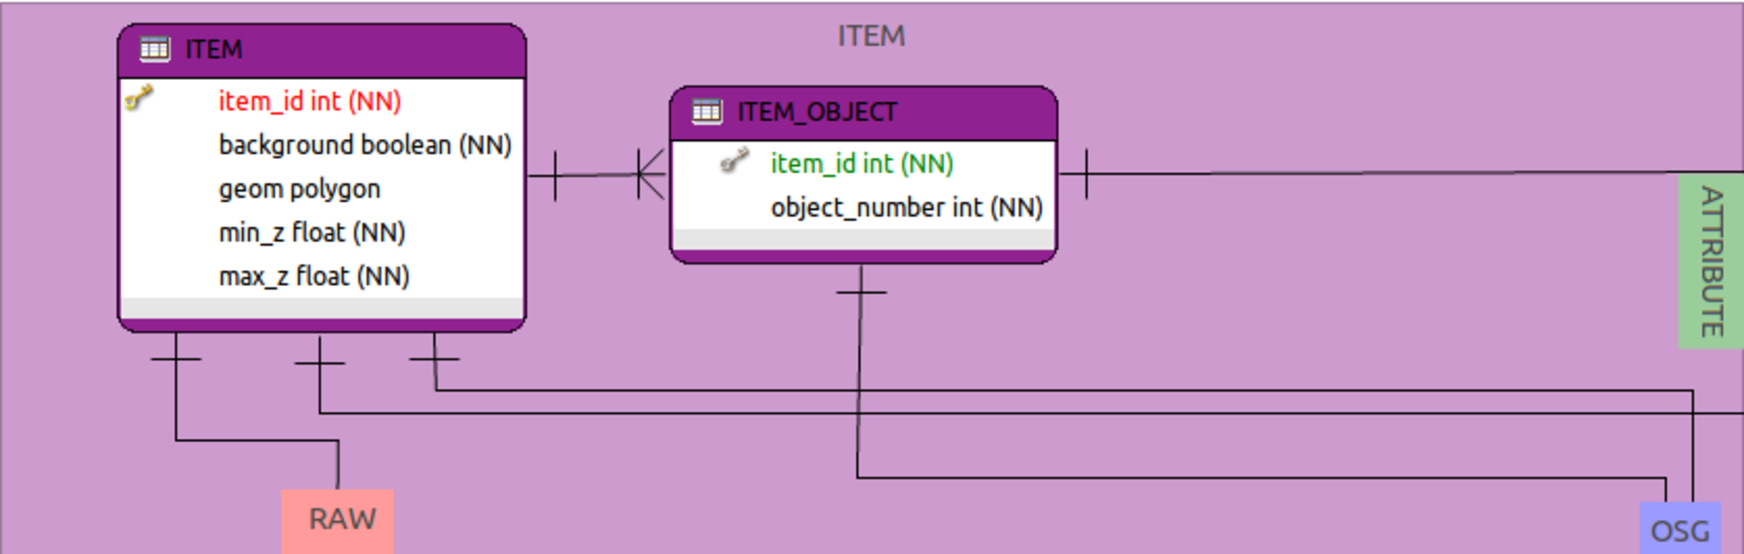
\includegraphics[scale=0.35]{fig/database/ERDB_ITEM_conn.pdf}
\caption{Entity-Relationship diagram of category ITEM and indicated connections
with other categories.}
\label{fig:db_erdb_item}
\end{figure}

\subsubsection{RAW}
The {\em RAW} category contains all the references to \textit{raw data} gathered for the items.
The most important meta-data is the location in the Data structure (Section~\ref{sec:data_structure}),
stored in the {\em abs\_path} field of the {\em raw\_data\_items}. These data can be either point clouds (PC),
meshes (MESH) or pictures (PICTURE). Each of these types is represented by a separate
table with the specific for that data type properties. The {\em RAW} category is
related to the derived data categories {\em OSG} and {\em POTREE} as indicated on
Figure~\ref{fig:db_erdb_raw}.

\begin{figure}[H]
\centering
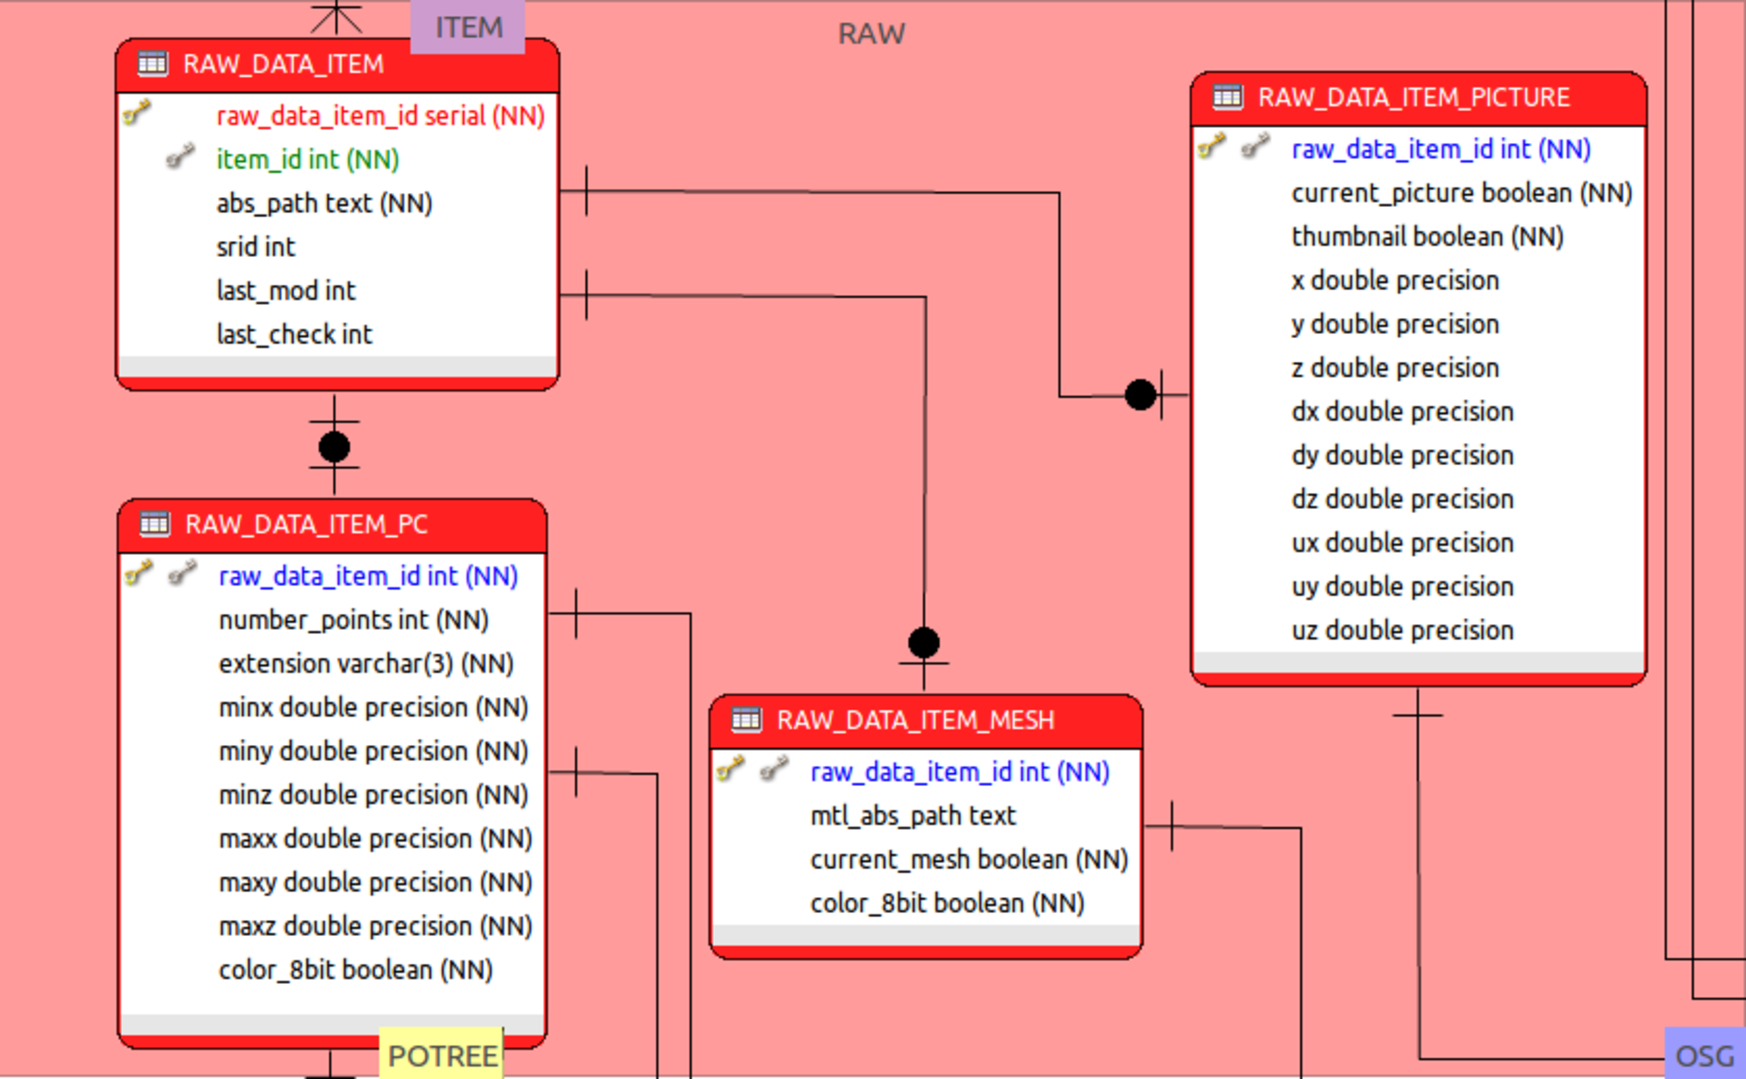
\includegraphics[scale=0.35]{fig/database/ERDB_RAW_conn.pdf}
\caption{Entity-Relationship diagram of category {\em RAW} and indicated connections
with other categories.}
\label{fig:db_erdb_raw}
\end{figure}

\subsubsection{OSG}
The {\em OSG} category contains the references of the OSG \textit{converted data} used for the
desktop based viewer. Figure \ref{fig:db_erdb_osg} depicts its relationships with the rest of related categories, i.e. the RAW data category
(from where it is derived) and the ITEM category. The tables in this category
reflect the possible data types: point clouds, meshes and pictures. This category contains meta-data of their data location in the Data Structure (Section~\ref{sec:data_structure}) as well as information needed for the \textit{visualization}, most importantly the information about the position of the various sites in the background.

\begin{figure}[H]
\centering
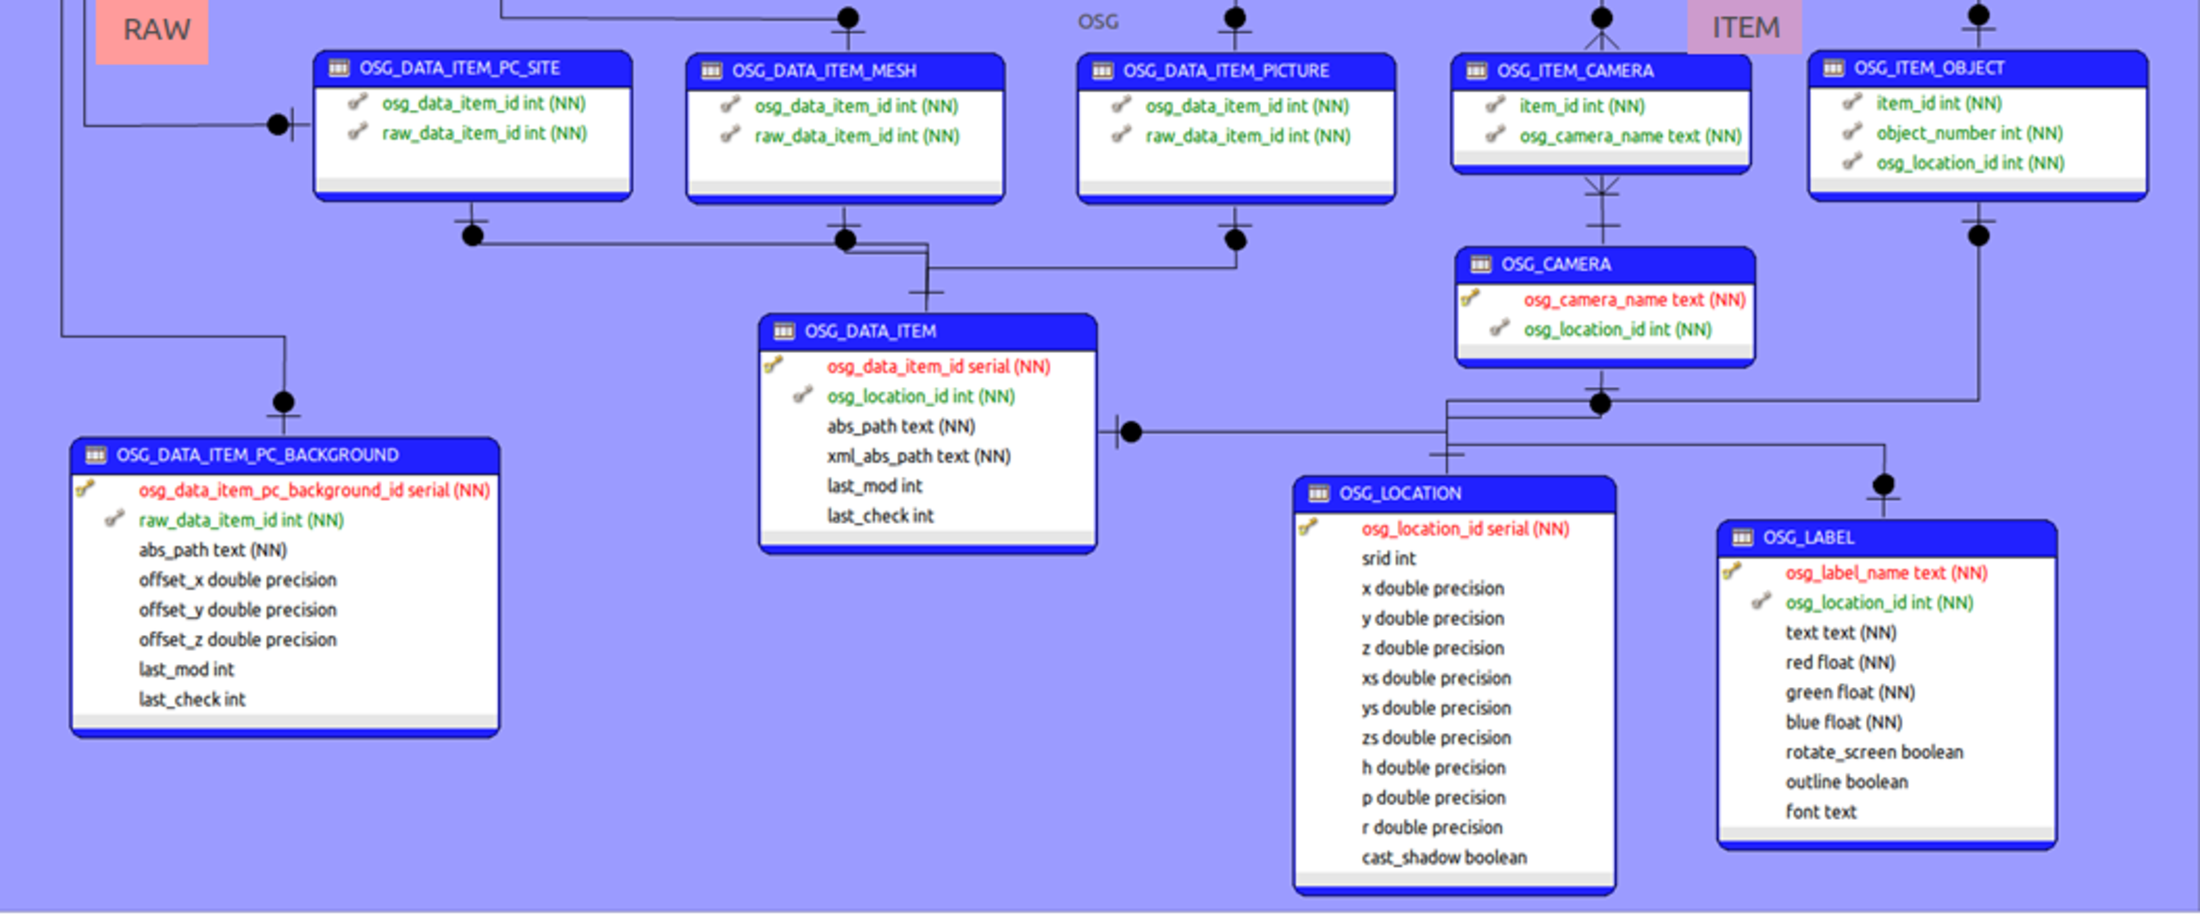
\includegraphics[scale=0.35]{fig/database/ERDB_OSG_conn.pdf}
\caption{Entity-Relationship diagram of category {\em OSG} and indicated connections
with other categories.}
\label{fig:db_erdb_osg}
\end{figure}

\subsubsection{POTREE}
The {\em POTREE} category is illustrated on Figure \ref{fig:db_erdb_potree}. It
is related only to the {\em RAW} category from which it is derived. Since the POTree web viewer only displays point cloud data only this type of data is considered. In this category we store meta-data information about the location of the data in the Data Structure (Section~\ref{sec:data_structure}) and the parameters used for the data conversion ({\em number\_levels}).

\begin{figure}[H]
\centering
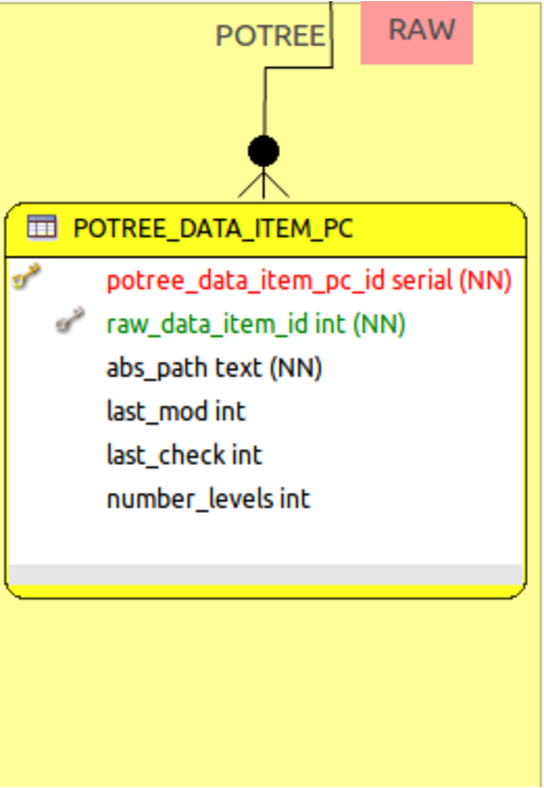
\includegraphics[scale=0.35]{fig/database/ERDB_POTREE_conn.pdf}
\caption{Entity-Relationship diagram of category {\em POTREE} and indicated
connections with other categories.}
\label{fig:db_erdb_potree}
\end{figure}

\subsection{Attribute data}
The attribute part of the DB is represented only by one category, {\em ATTRIBUTE}
(Figure \ref{fig:db_erdb_attribute}). It is connected only to the {\em ITEM} category.
These are the information collected during the field work and are primarily of research
interest to the archaeologists as it contains all domain-related data enabling browsing
and filtering of sub-parts of the data of interest.

\begin{figure}[H]
\centering
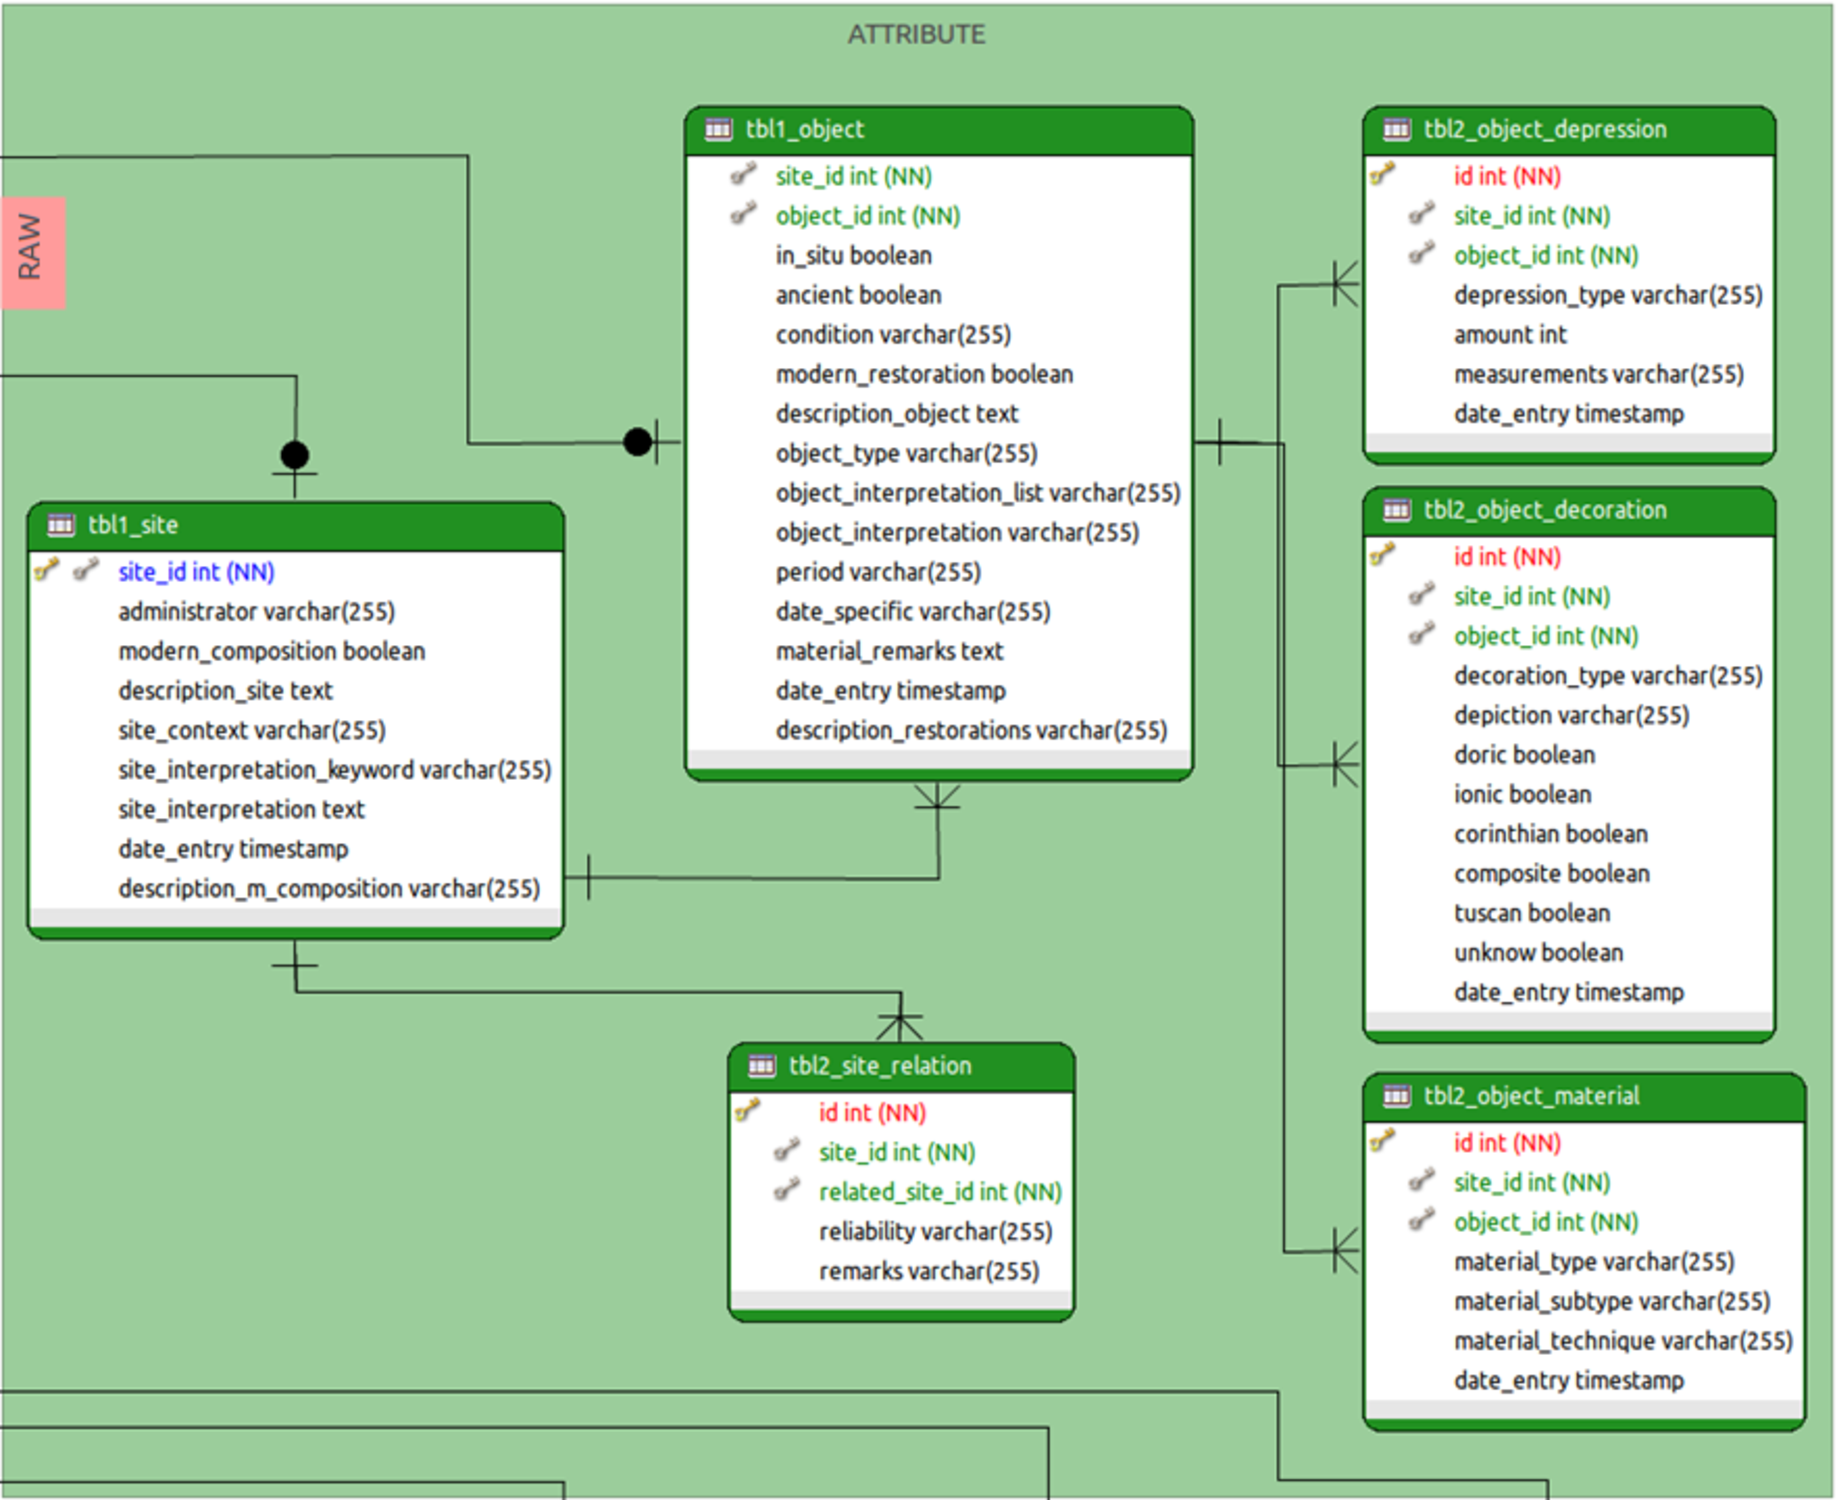
\includegraphics[scale=0.35]{fig/database/ERDB_ATTRIBUTE_conn.pdf}
\caption{Entity-Relationship diagram of category {\em ATTRIBUTE} and indicated
connections with other categories.}
\label{fig:db_erdb_attribute}
\end{figure}

\subsection{Database scripts}
\label{sec:dbscripts}
There is a collection of scripts to manipulate the data in the database. Like for the data storage scripts, it is important to notice that operations modifying the database must be run with \textit{pattydat} user.

\subsubsection{Updating the DB}
After any change in the directory structure (adding or removing raw data item, generating converted data for OSG or POTree) the user must run the script \textit{UpdateDB.py} in order to let the DB know about the recent changes.

\subsubsection{Other database scripts}
There are other scripts for updating the footprints, the altitude ranges, the attribute data and to create the database but these are only meant for the administrators and not for regular users so its description is not covered in this manual.